\documentclass{article}
%\documentclass[journal]{IEEEtran}
%\documentclass{report}
%\documentclass{ActaOulu}

\usepackage[pdftex,bookmarks=true]{hyperref}
\usepackage[pdftex]{graphicx}
\usepackage[utf8]{inputenc}
\usepackage{cite}

\begin{document}

\title{Introduction to the alibava setup}
\author{Arne-Rasmus Dr\"ager}

\maketitle

\begin{abstract}
The alibava setup can be used to measure the influence of radiation on silicon strip detectors. This note gives an introduction to the setup and a brief explenation how to use it..
\end{abstract}


%\chapter{First Chapter}

\section{Introduction}

High energy particle experiments demand very powerful machines with high instantaneous luminosities. In order to operate detectors at this high intensities new materials have to be developed that withstand very harsh radiation conditions. The alibava setup is one important setup in the chain of developing new radiation hard silicon strip detectors for the CMS experiments so called phase two upgrade. The setup can be used to measure the charge collection efficiency at different temperatures different voltages with either a $\beta$ strontium 90 source or a laser. The focus of this document is neither meant to provide an introductory on silicon micro-strip detectors nor on the operation of the electronics of setup. Information on this can be found in Ref. \cite{Silicon_Microstrip_dectectors_anna_peisert} 
\section{Setup}
In order to start measuring eight devices need to be turned on. The order in which the devices are turned on does not matter however they all need to be turned on before starting the alibava control software.  All devices are listed in table \ref{tab:devices} and are shown in figure \ref{fig:MainUnits},\ref{fig:CurrentAndVoltageTrigger}.
\begin{table}[htb]
\begin{center}
    \begin{tabular}{|l|l|l|}
        \hline
	No. & Device Name		& Function	\\  \hline
        1 & Keithley 6517A		& Bias voltage supply and current measurement detector 		 \\
        2 & Ortec Model 401B		& Power for trigger		\\ 
        3 & TDK-Lambda			& Voltage supply for the peltier element		 \\ 
        4 & Keithley 2700		& Temperature monitor 		 \\ 
        5 & Relay box			& Relay box for the setup		 \\ 
        6 & Alibava			& Alibava box		 \\ 
        7 & OWIS			& Driver for the table with the detector		 \\ 
        8 & Lambda			& Heat exchanger for the peltier element		 \\ 
        9 & Two valves			& Dry air supply need when cooling active (optional) \\
        \hline

    \end{tabular}
\caption{Table of all devices that need to be turned on.}
\end{center}
\label{tab:devices}
\end{table}
The detector to be measured needs to be wireboned and fixed on a so called daughter-board which includes the readout chips. Fig.\ref{fig:InsideTheBox} shows a picture of an installed daughter-board with an detector wireboned on it. Three cables need to be connected: The power supply for the bias voltage , the heat sensor(round cable) and the big thin cable connecting the daughter-board to the alibava box.
In order to record measurements using the $\beta$ strontium 90 source Michael or somebody with radiation privileges needs to be present! (Use the 100MBk source for faster data gathering.)
After turning on all devices and opening the dry air valves (optional if cooling below room temperature) the alibava control software may be started (The password for the computer is: beetle11/09-03). 
\newline
\mbox{Make sure: NEVER TURN OF THE PC OR INSTALL ANY UPDATES!!!} 
\newline
Start the alibava control program with the conf file: 
\newline
 .dist/Debug/GNU-Linux-x86/alibava\_control /space/software/devconf.cfg
\newline
(Make sure the humidity usb is not connected!)
Here one can apply bias voltage, heat or cool the sensor, move the table and finally start measuring.
The measurements are than stored in:
\newline
 /space/measurement/\$DeviceName\$/\$DataTime\$/
\newline
An analyzation framework can be checked out from git using:
git clone HTTTP MISSING!!!

\begin{figure}[tbhn]
\begin{center}
\begin{tabular}{cc}
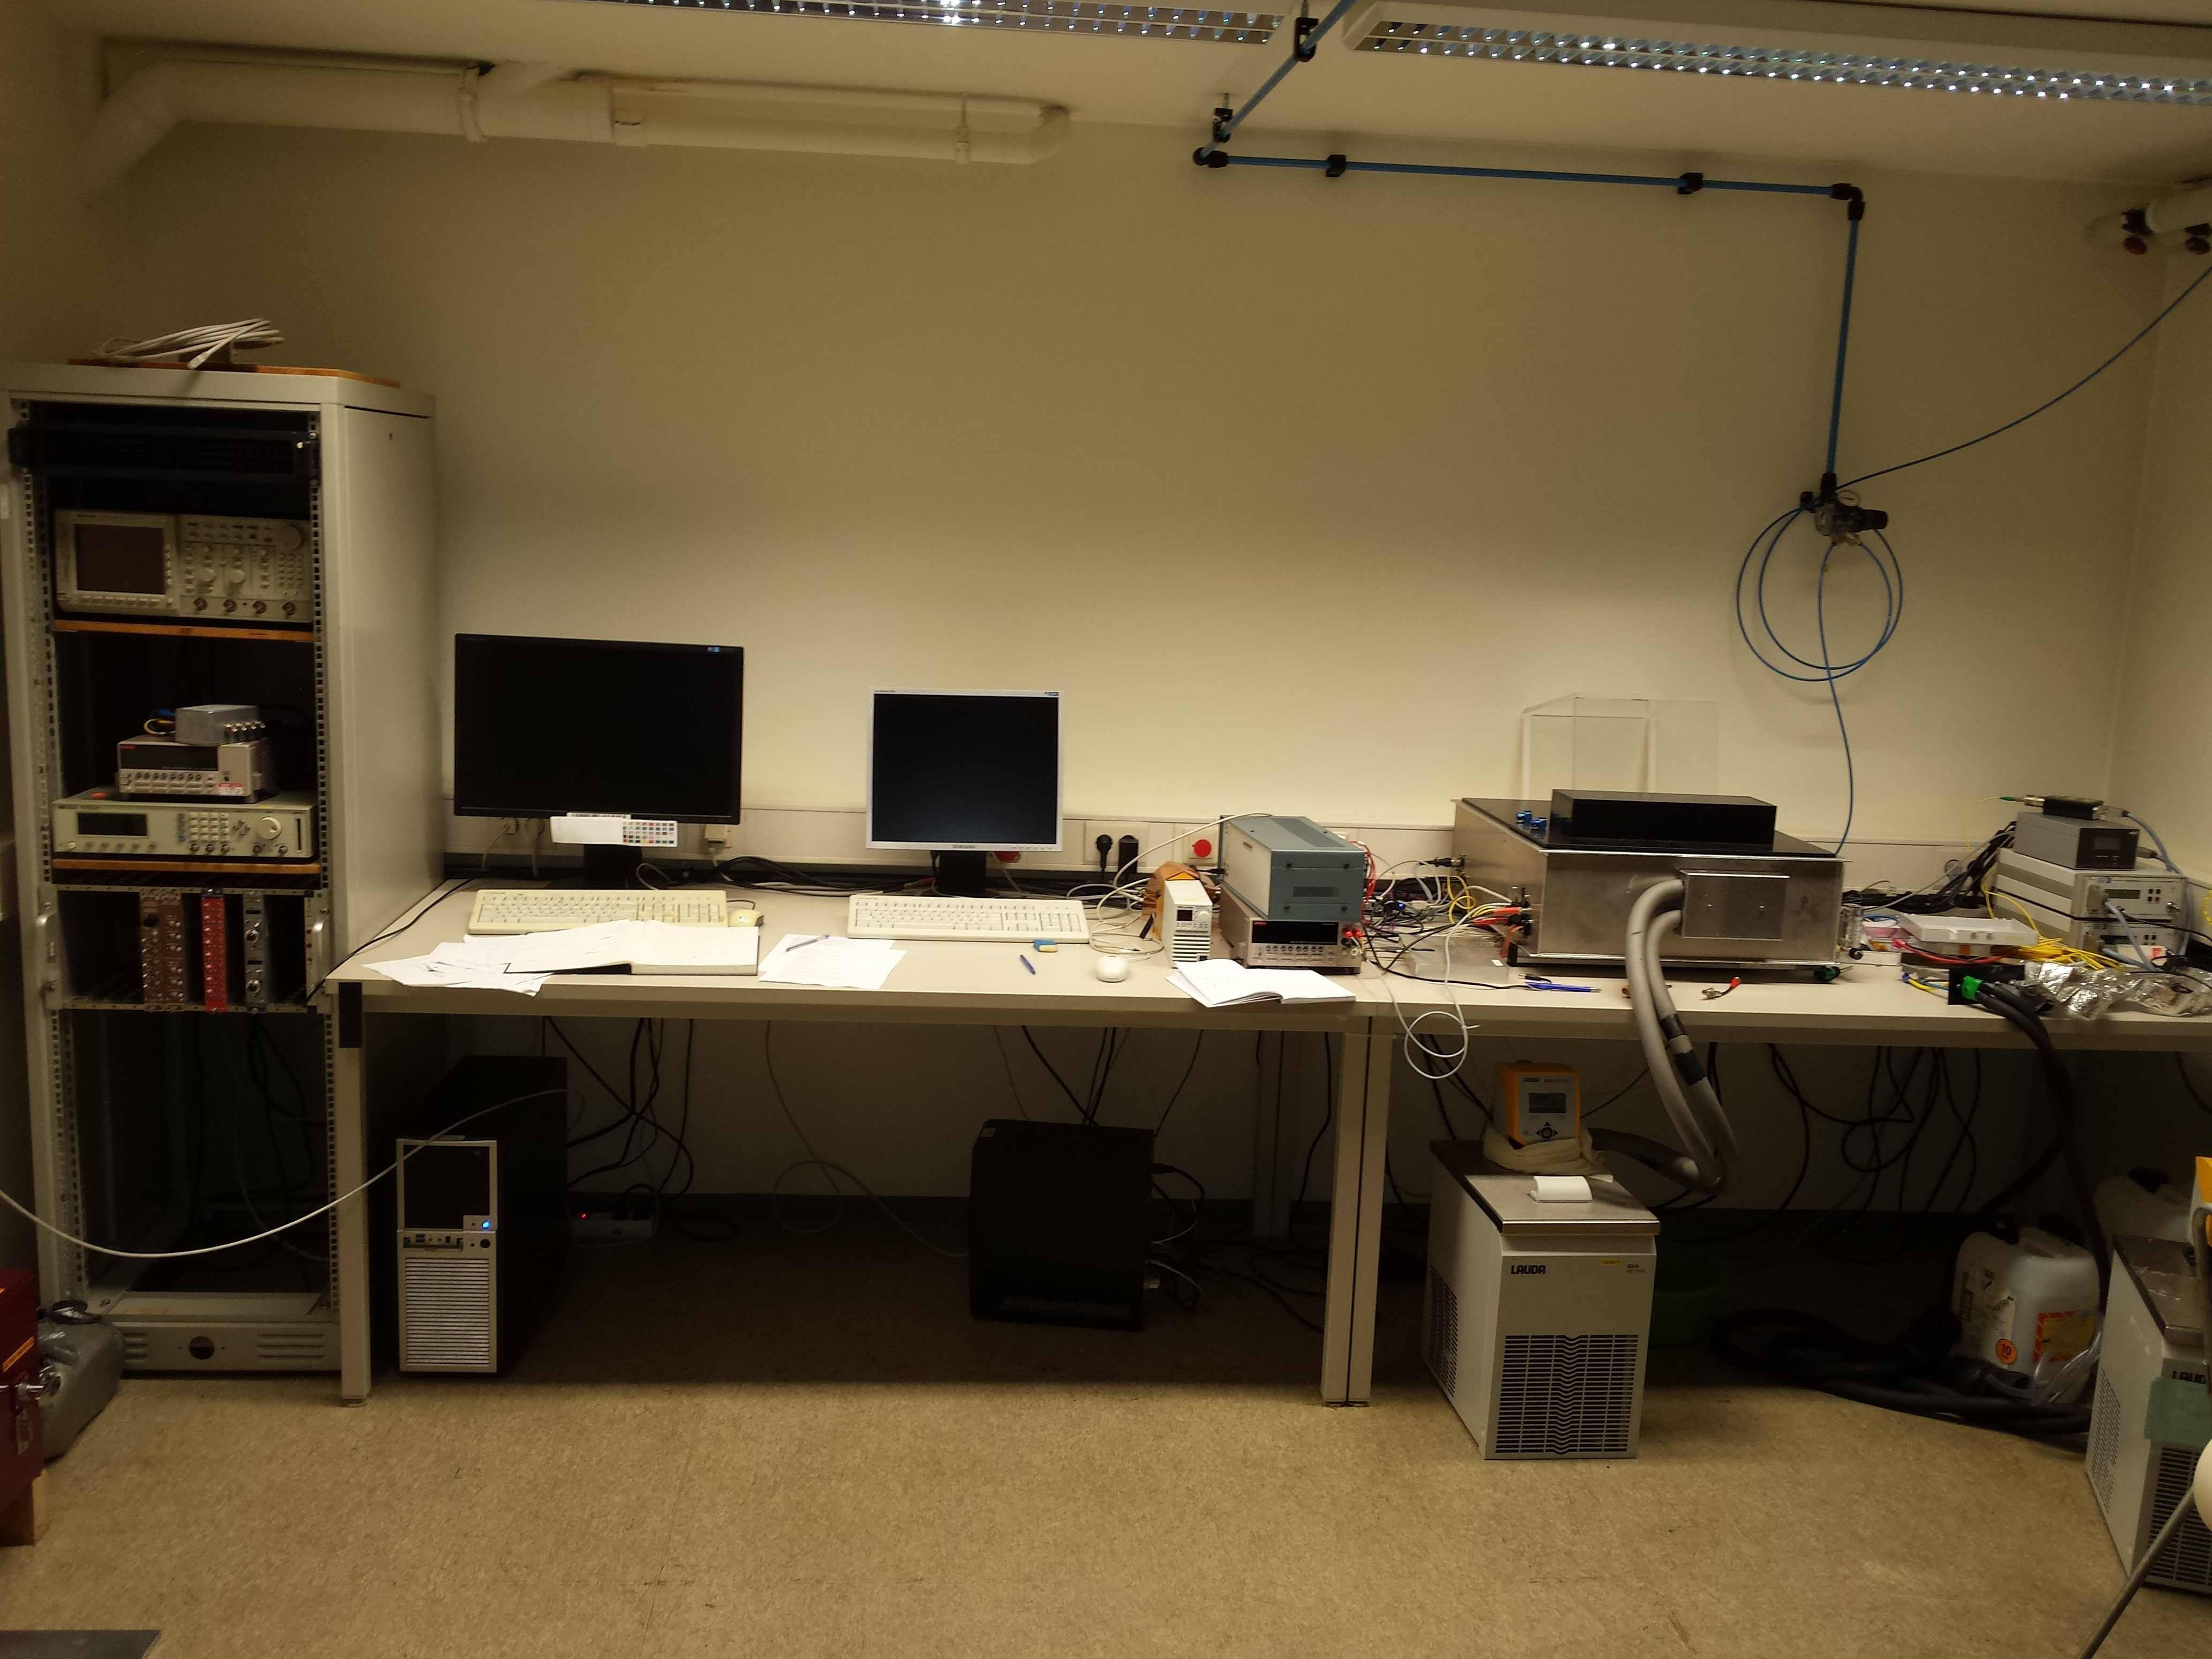
\includegraphics[width=0.49\textwidth]{pictures/FullSetup.jpg}
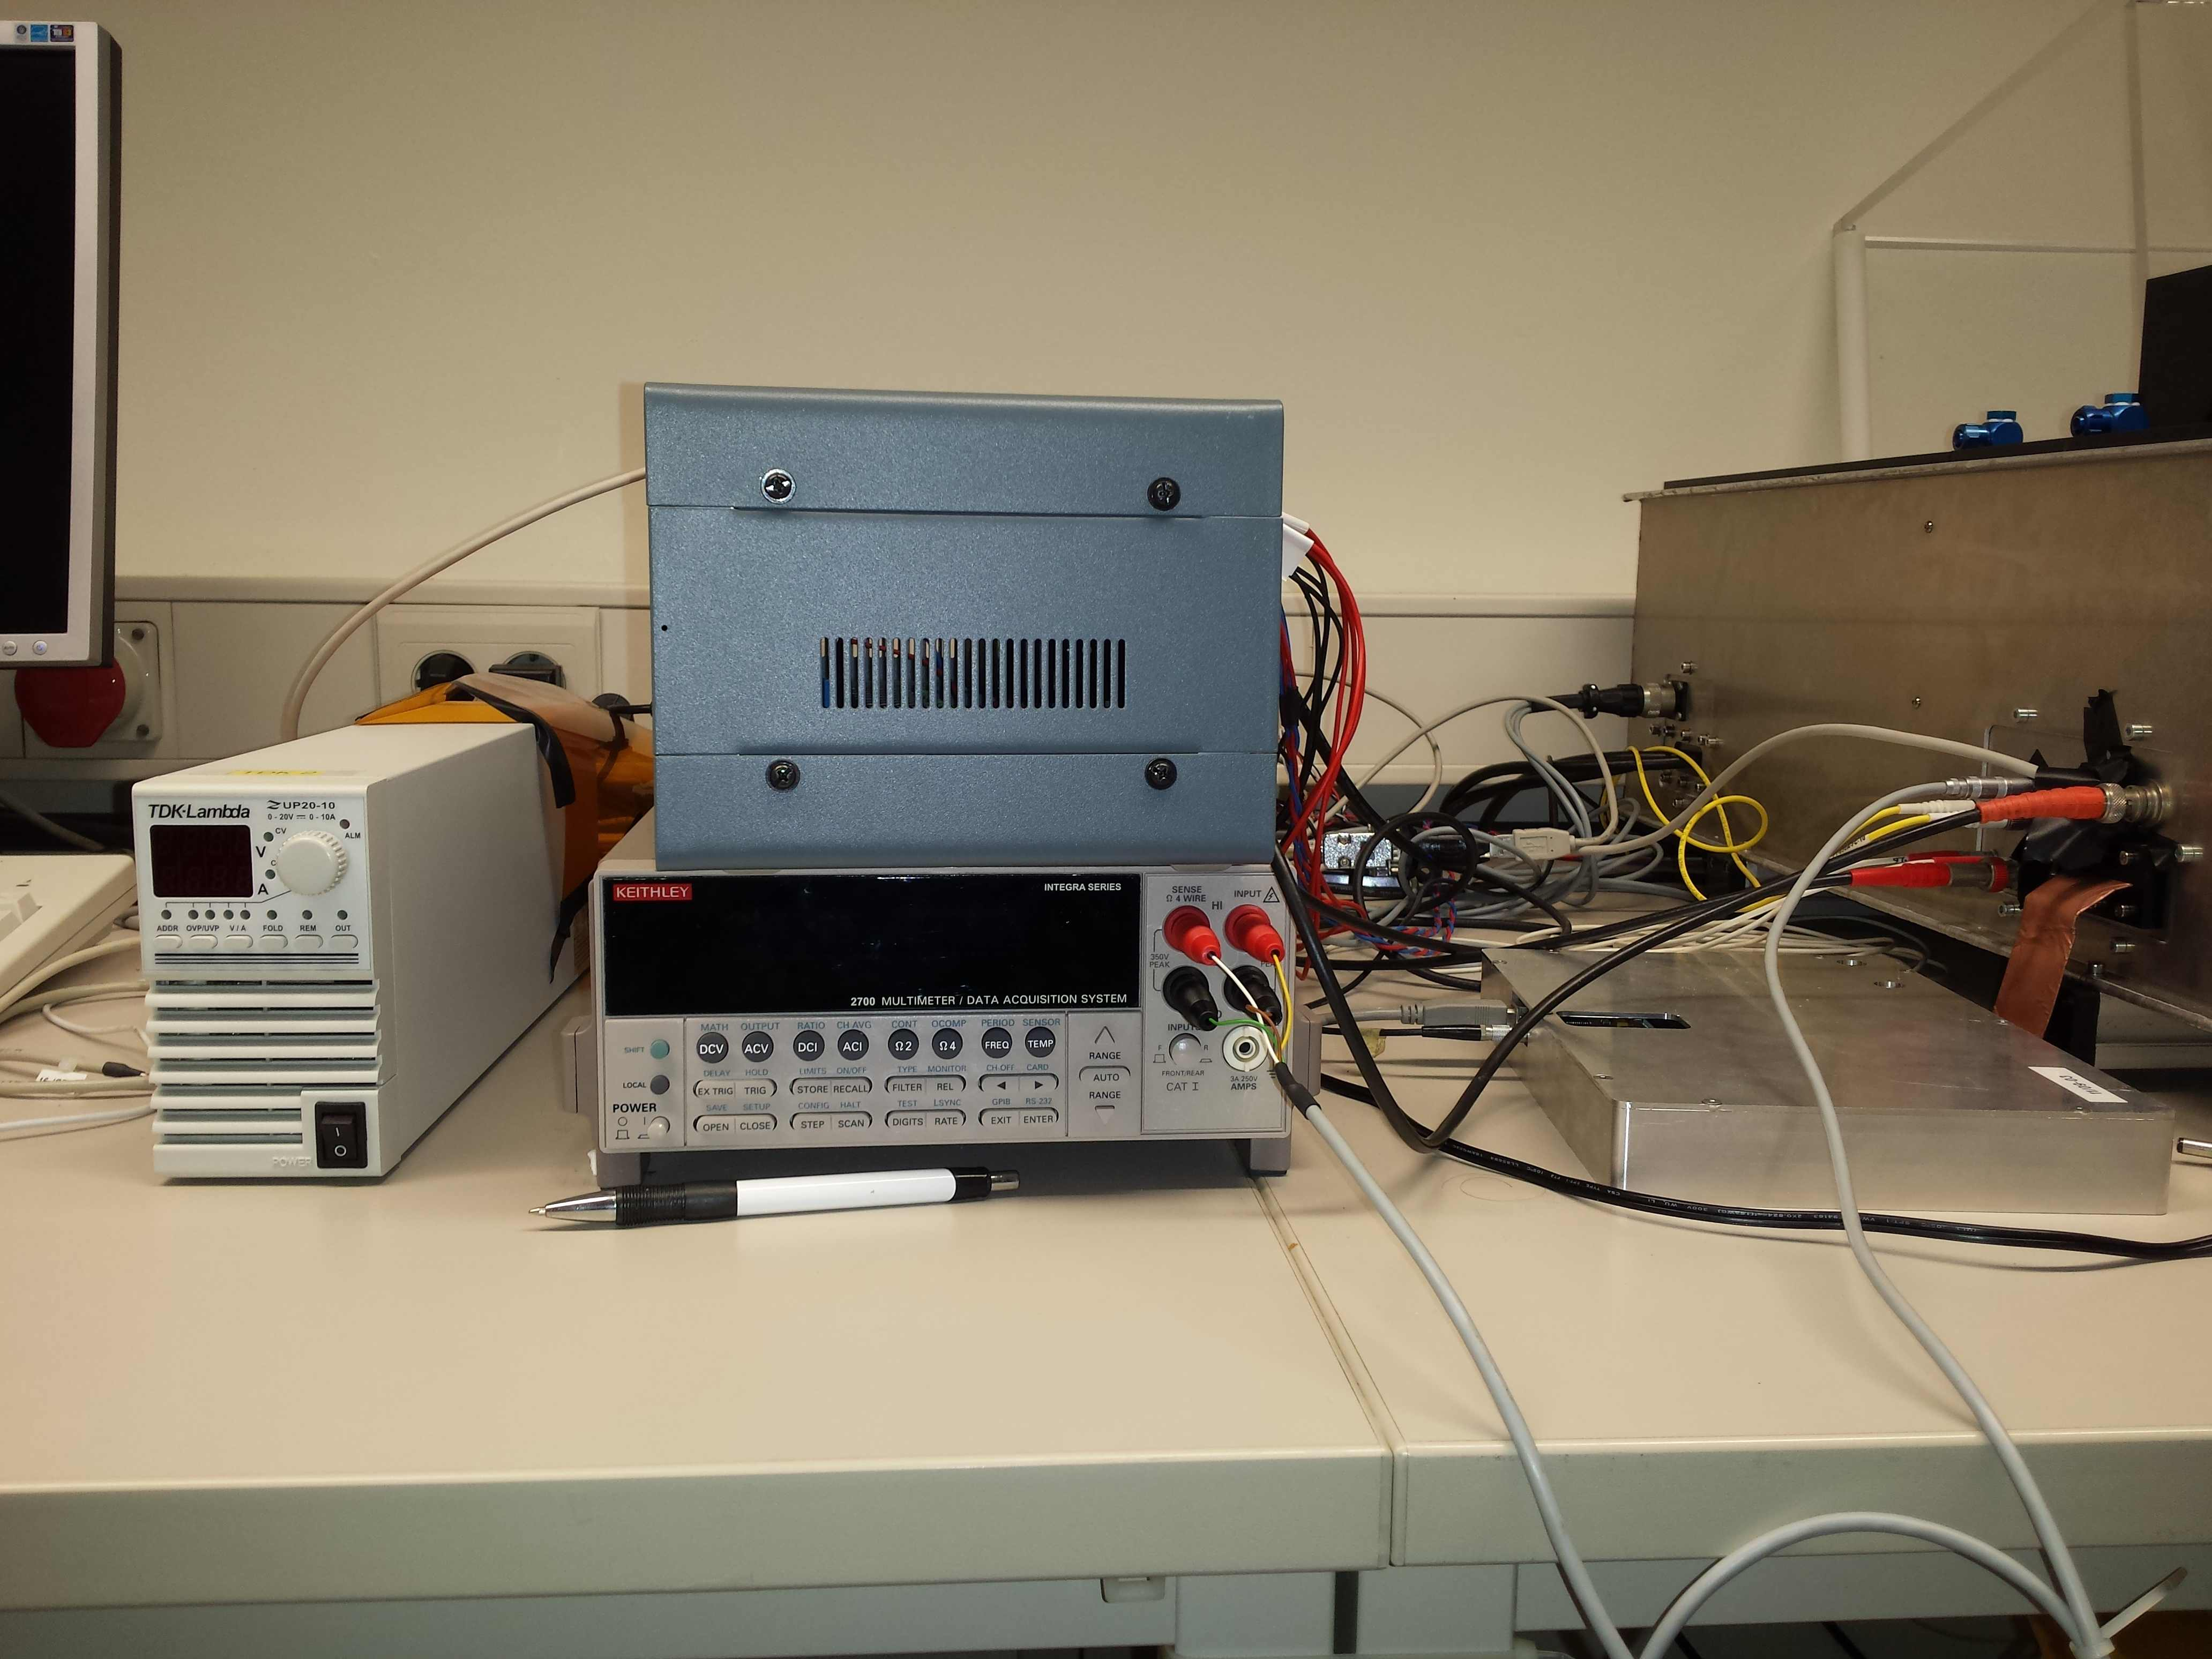
\includegraphics[width=0.49\textwidth]{pictures/MainUnits.jpg}
\end{tabular}
\end{center}
\caption{The left picture shows the full setup while the right shows (from left to right, top to bottom) the Voltage supply for the peltier element (3), relay box(5), temperature monitor(4) and the alibava box(6). The numbers in brackets correspond to table \ref{tab:devices}. }
\label{fig:MainUnits}
\end{figure}
\begin{figure}[tbhn]
\begin{center}
\begin{tabular}{c}
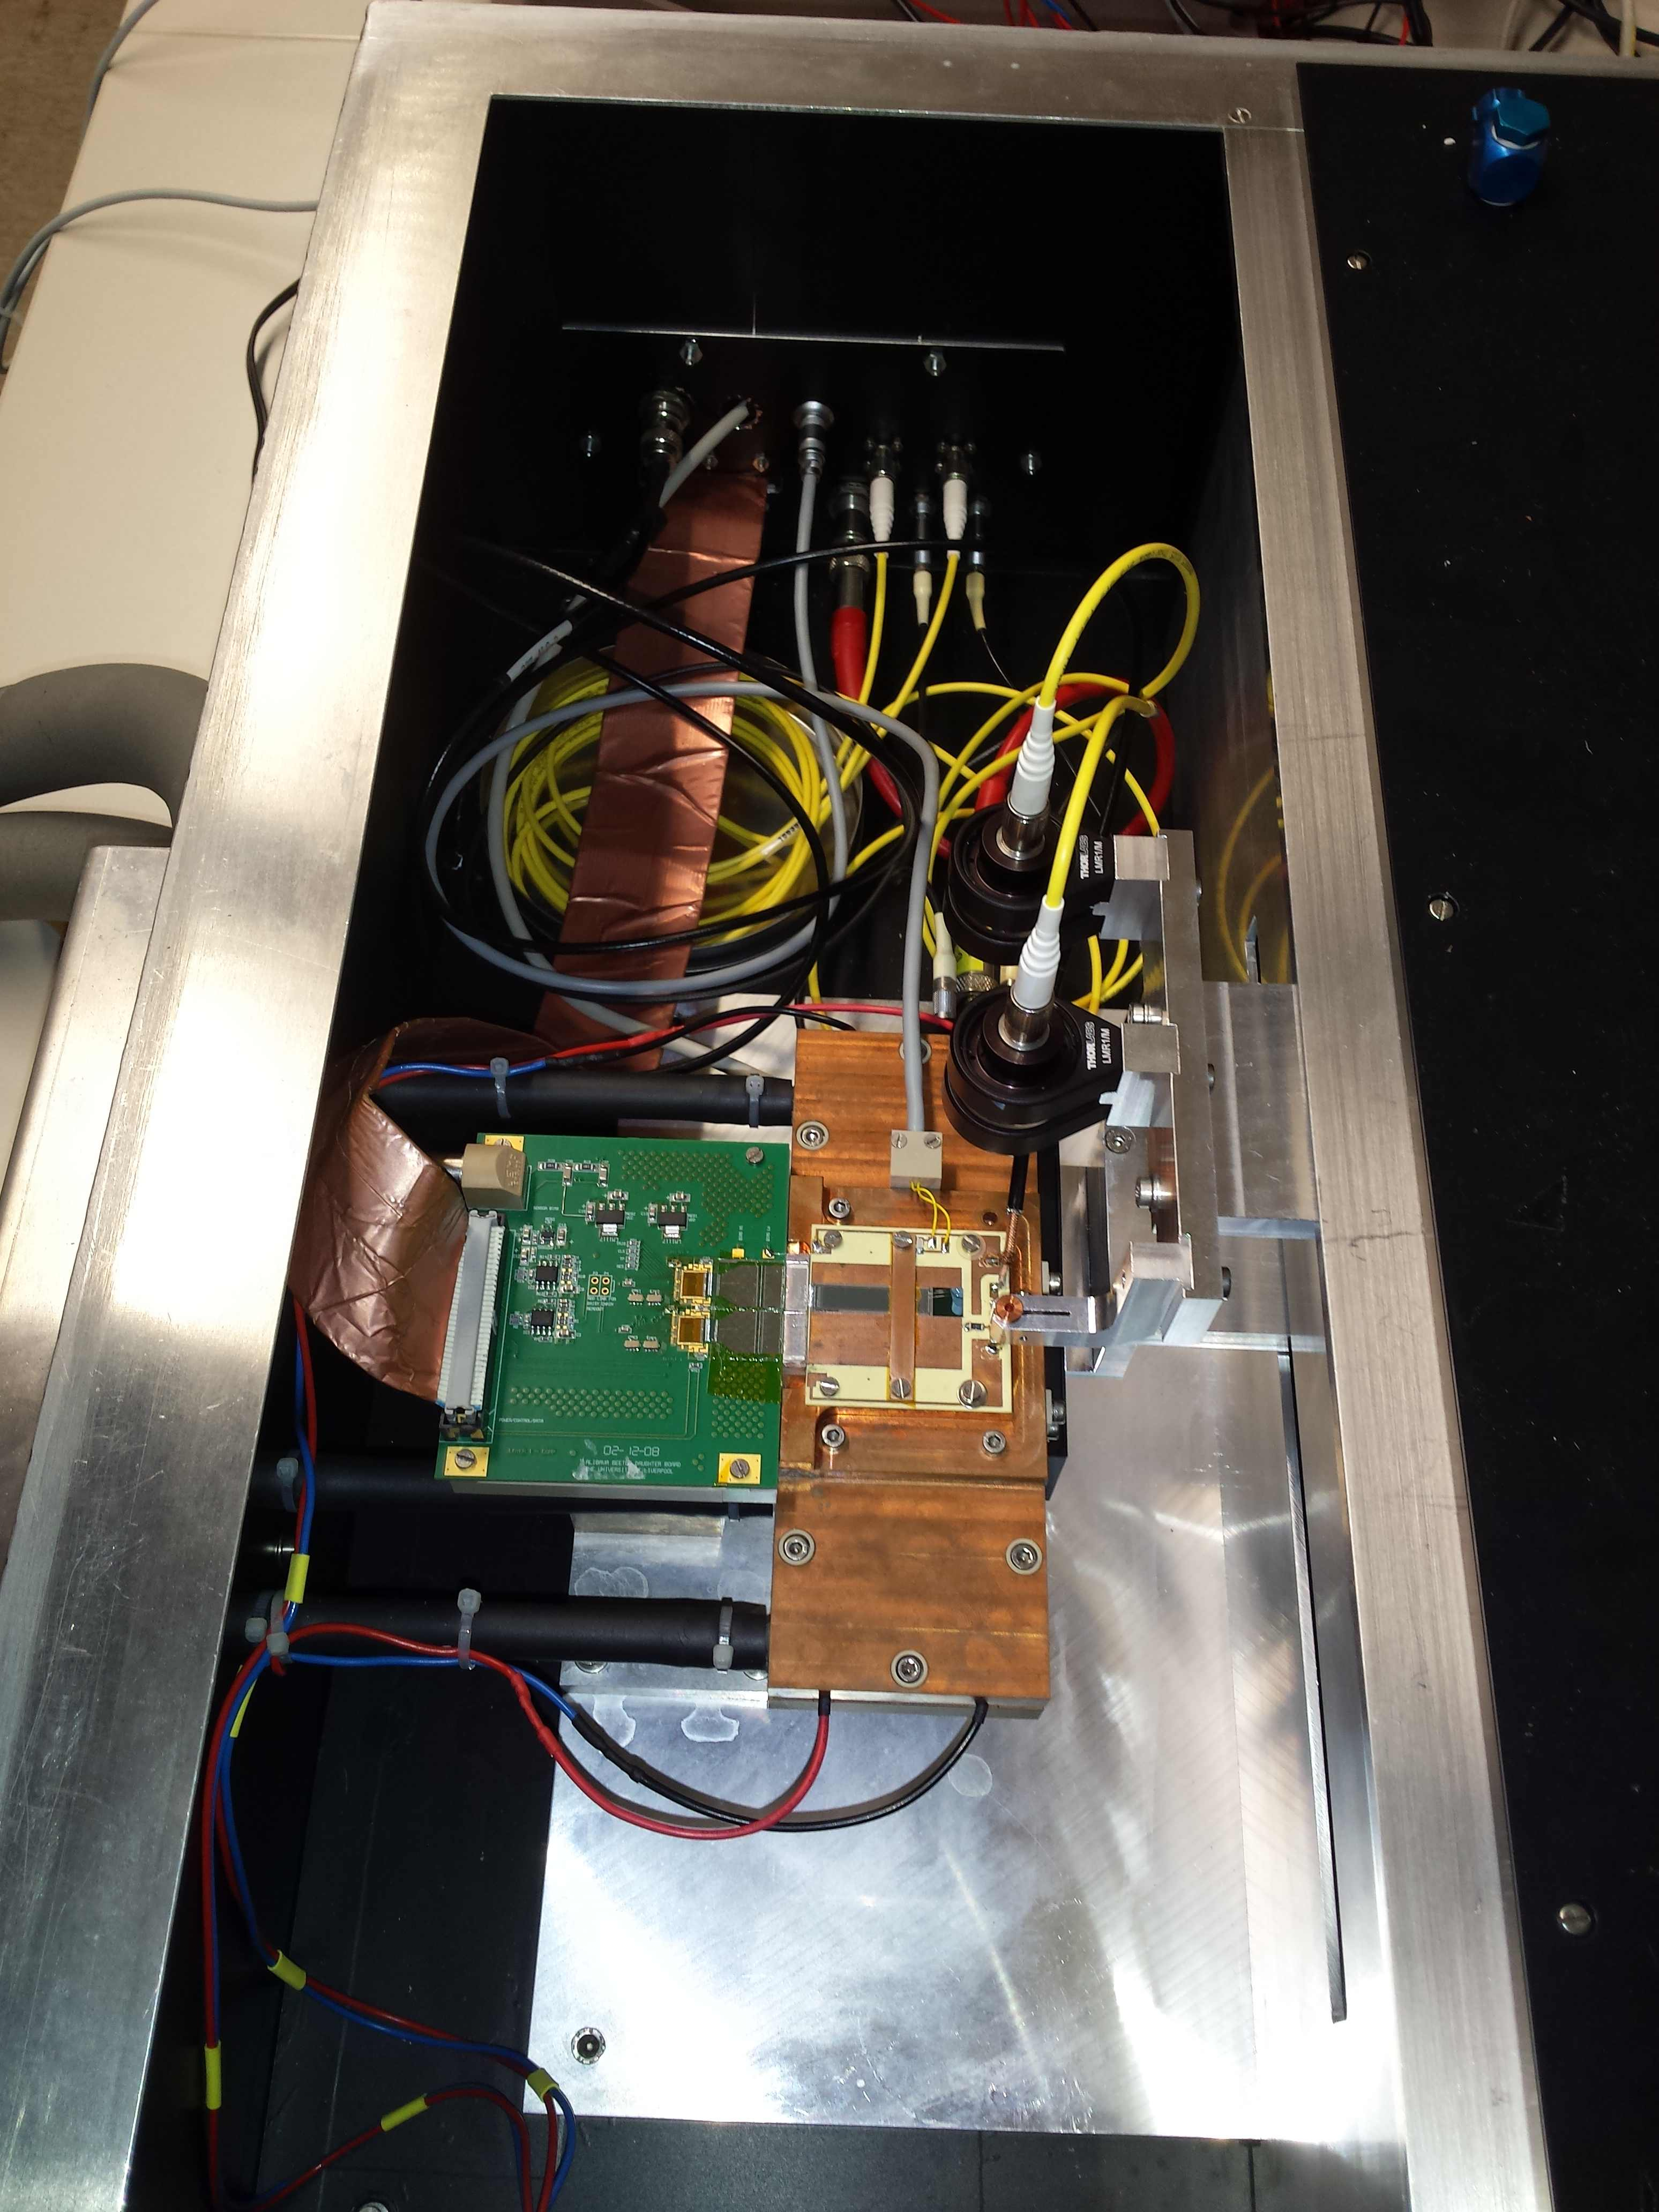
\includegraphics[width=0.98\textwidth]{pictures/InsideTheBox.jpg}
\end{tabular}
\end{center}
\caption{The interior of the measurement box (black) with a daughter-board and a detector on it can be seen in this picture. The extra isolated cable on the left side (big flat one) is connected to the alibava box(6) while the gray one with the two yellow end peaces connected the temperature sensor(4) and the black one connects the bias voltage to the detector(1).}
\label{fig:InsideTheBox}
\end{figure}
\begin{figure}[tbhn]
\begin{center}
\begin{tabular}{cc}
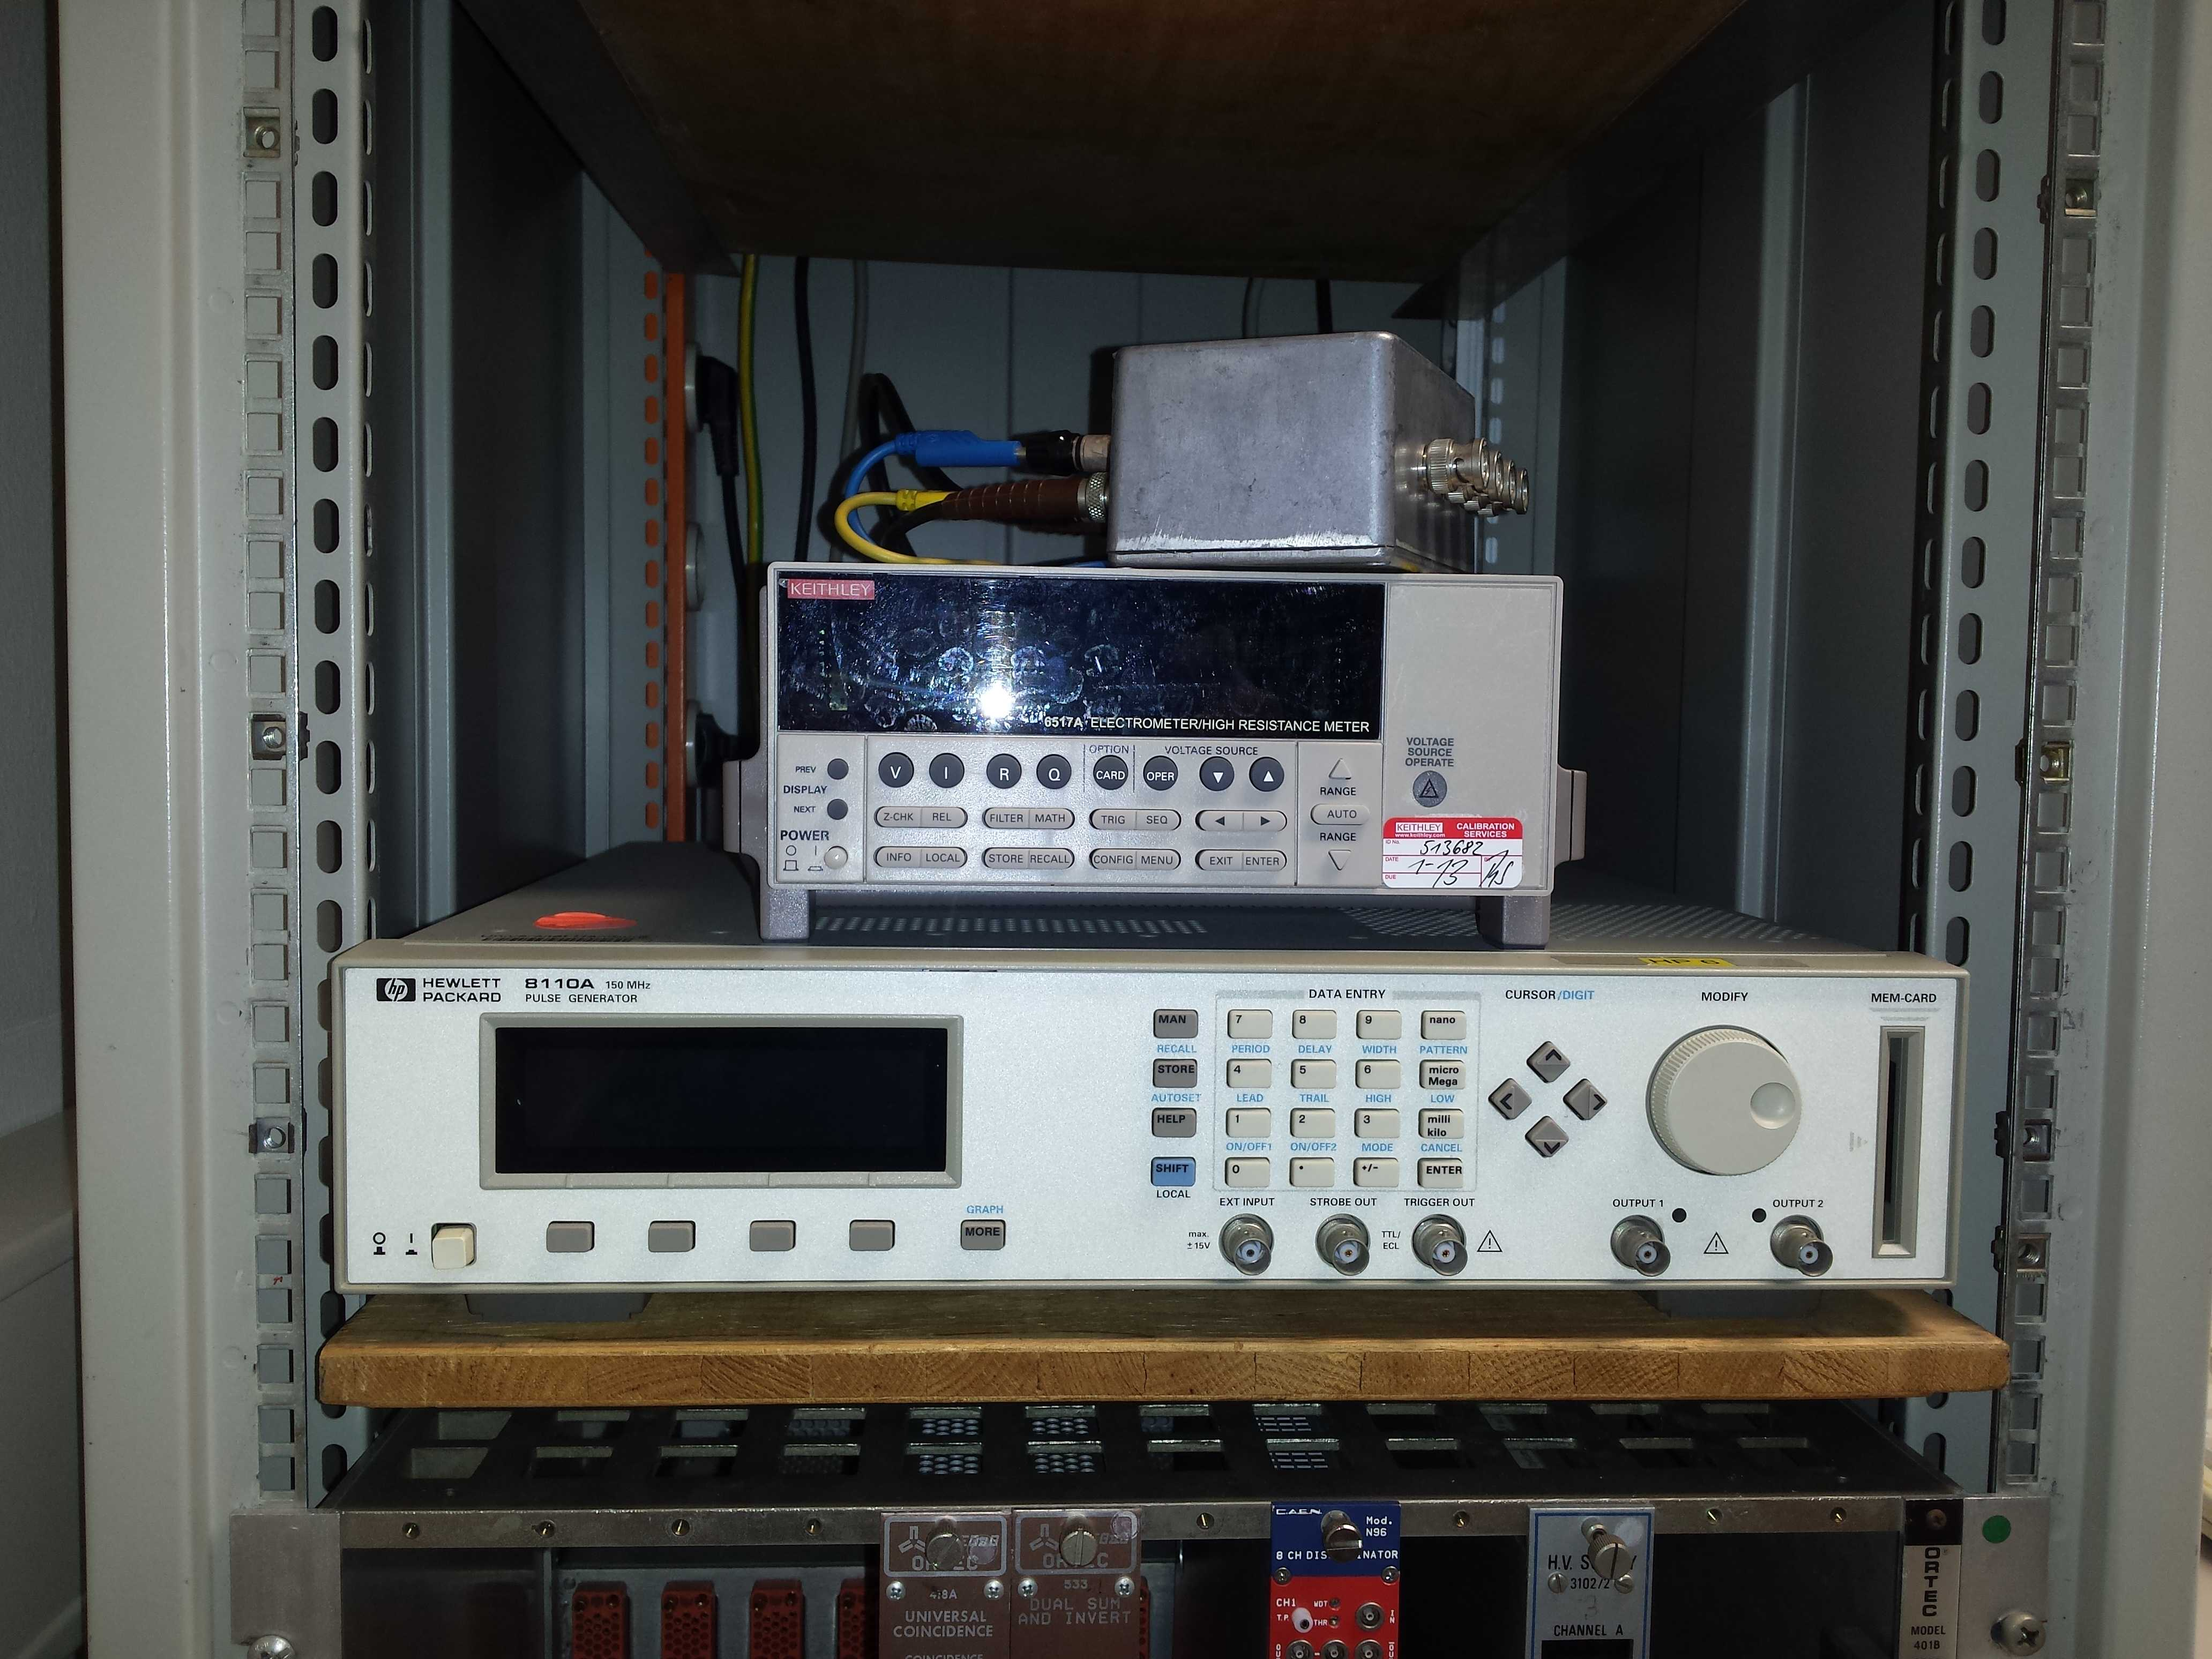
\includegraphics[width=0.49\textwidth]{pictures/CurrentAndVoltage.jpg}
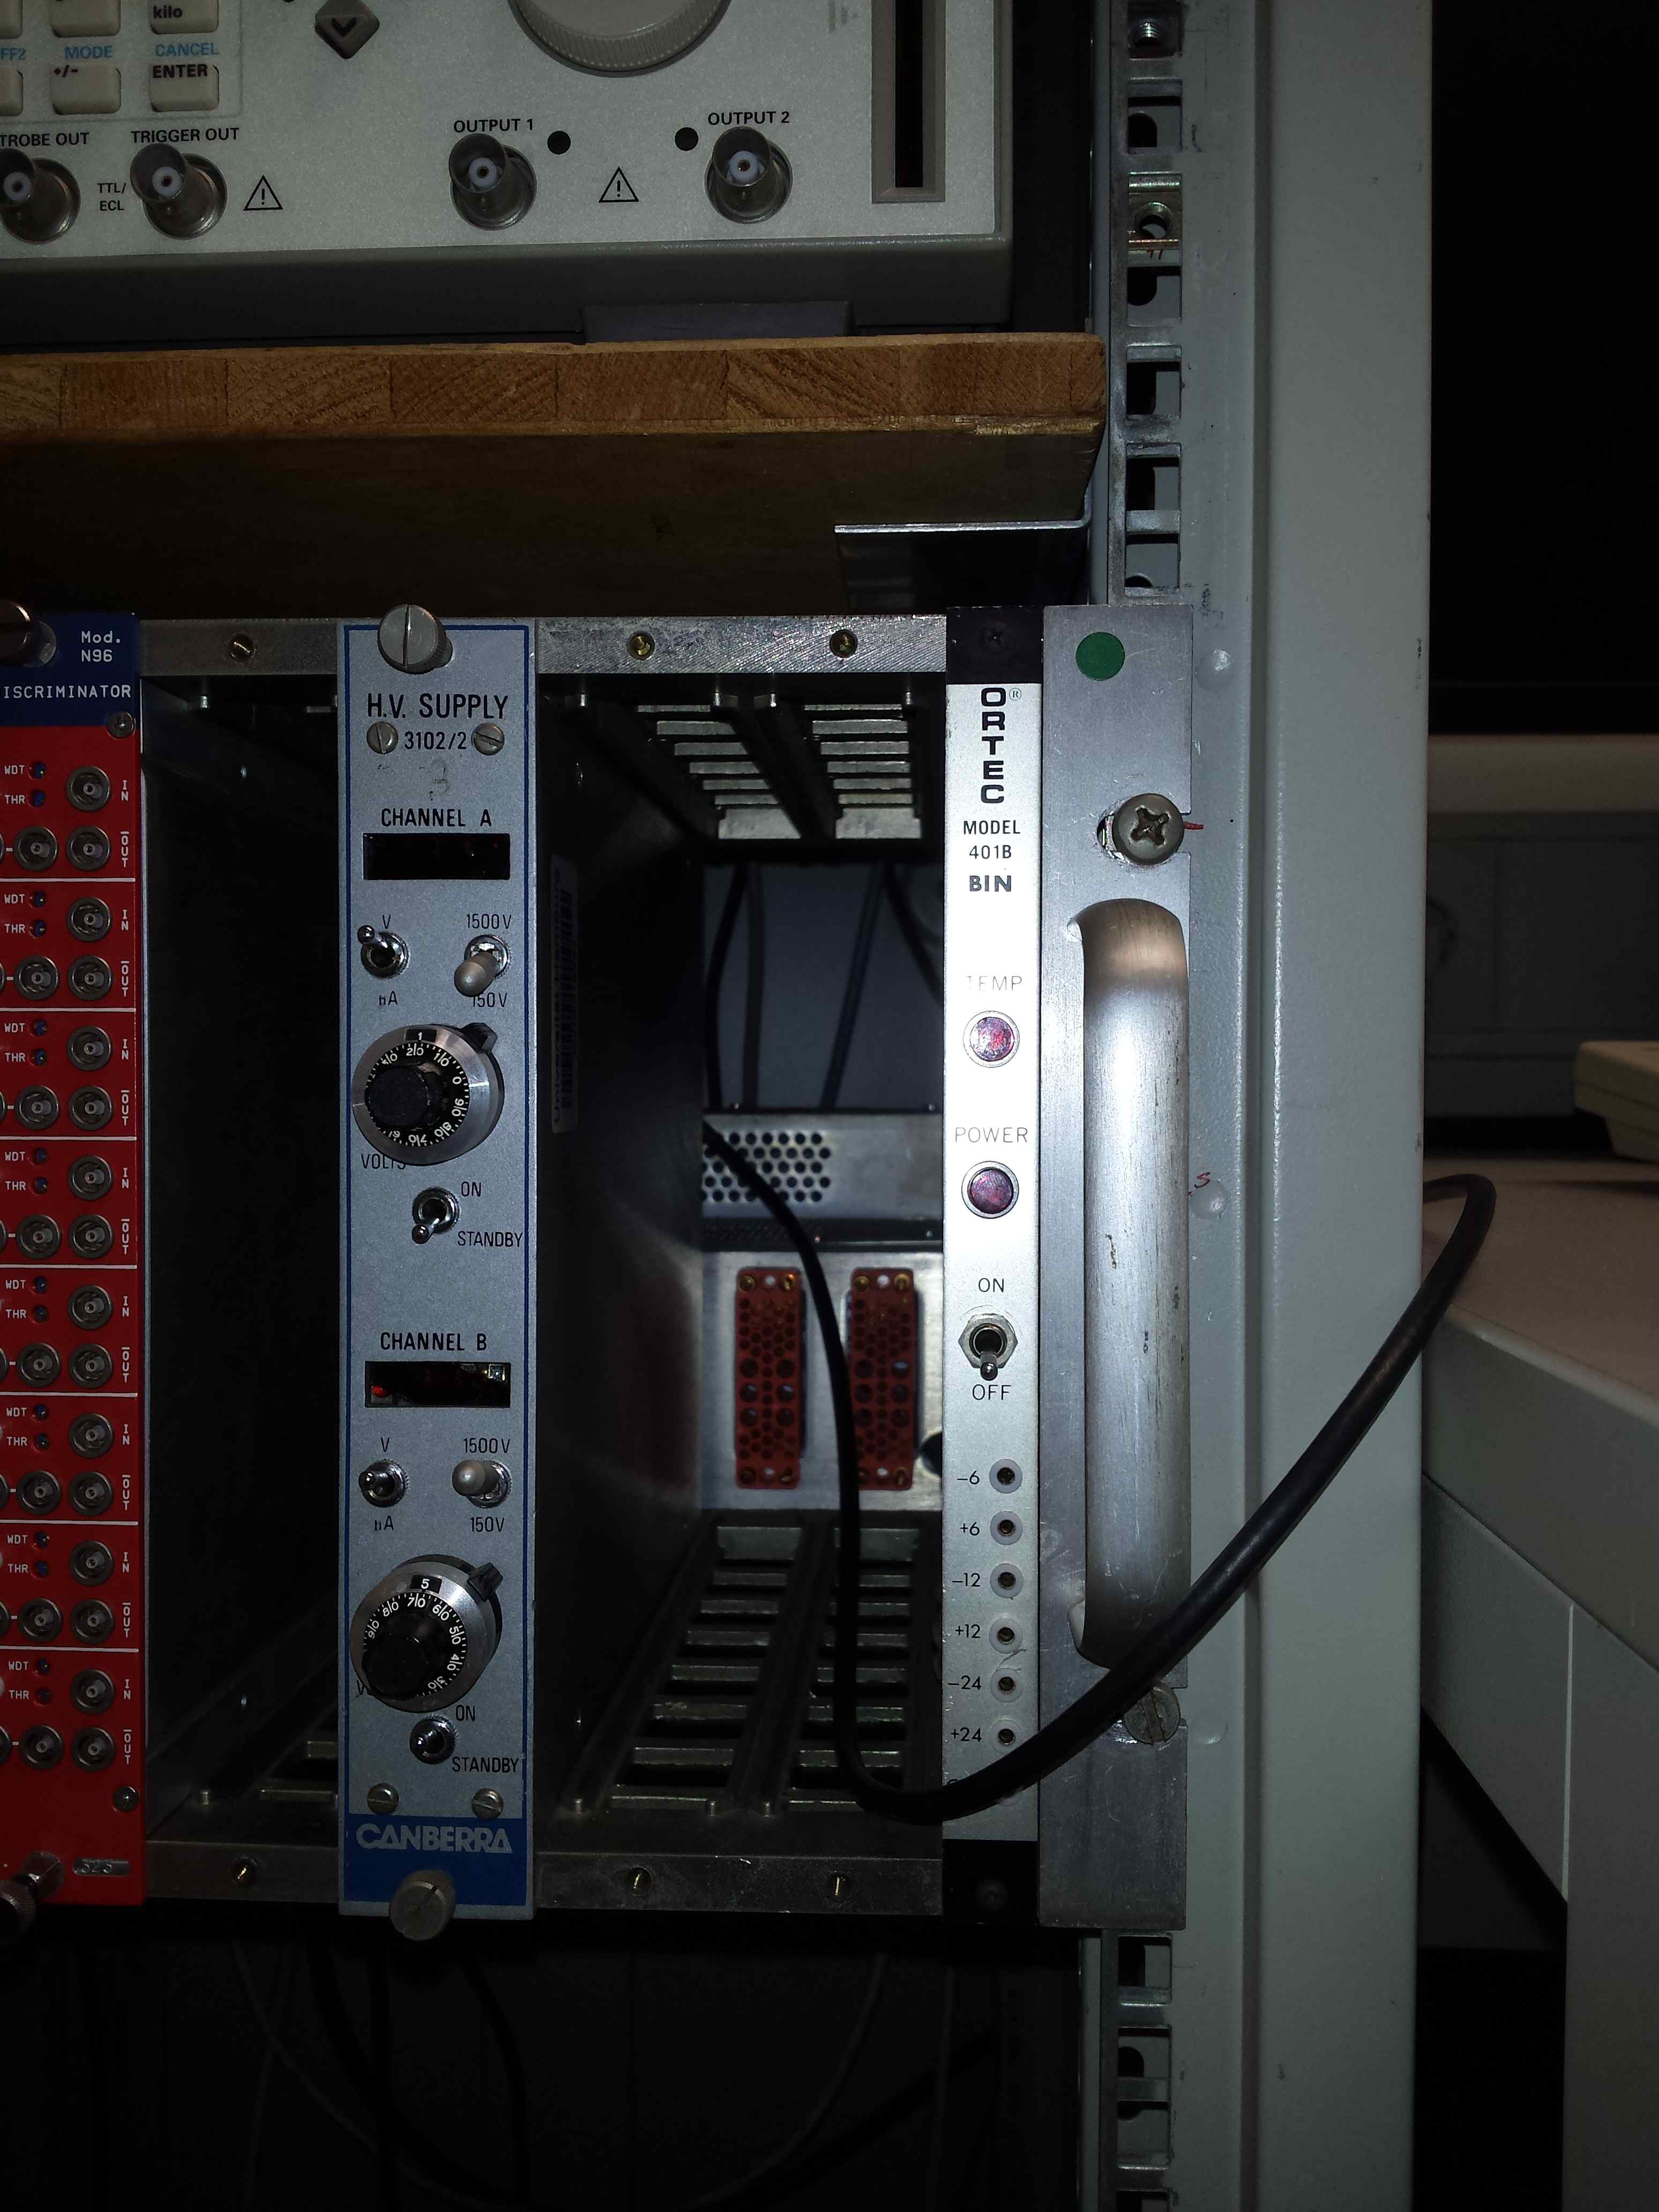
\includegraphics[width=0.49\textwidth]{pictures/Trigger.jpg}
\end{tabular}
\end{center}
\caption{The left picture shows the bias voltage and current supply for the detector(1), while on the right side the trigger power supply is shown(2). The numbers in brackets correspond to table \ref{tab:devices}. }
\label{fig:CurrentAndVoltageTrigger}
\end{figure}
\begin{figure}[tbhn]
\begin{center}
\begin{tabular}{cc}
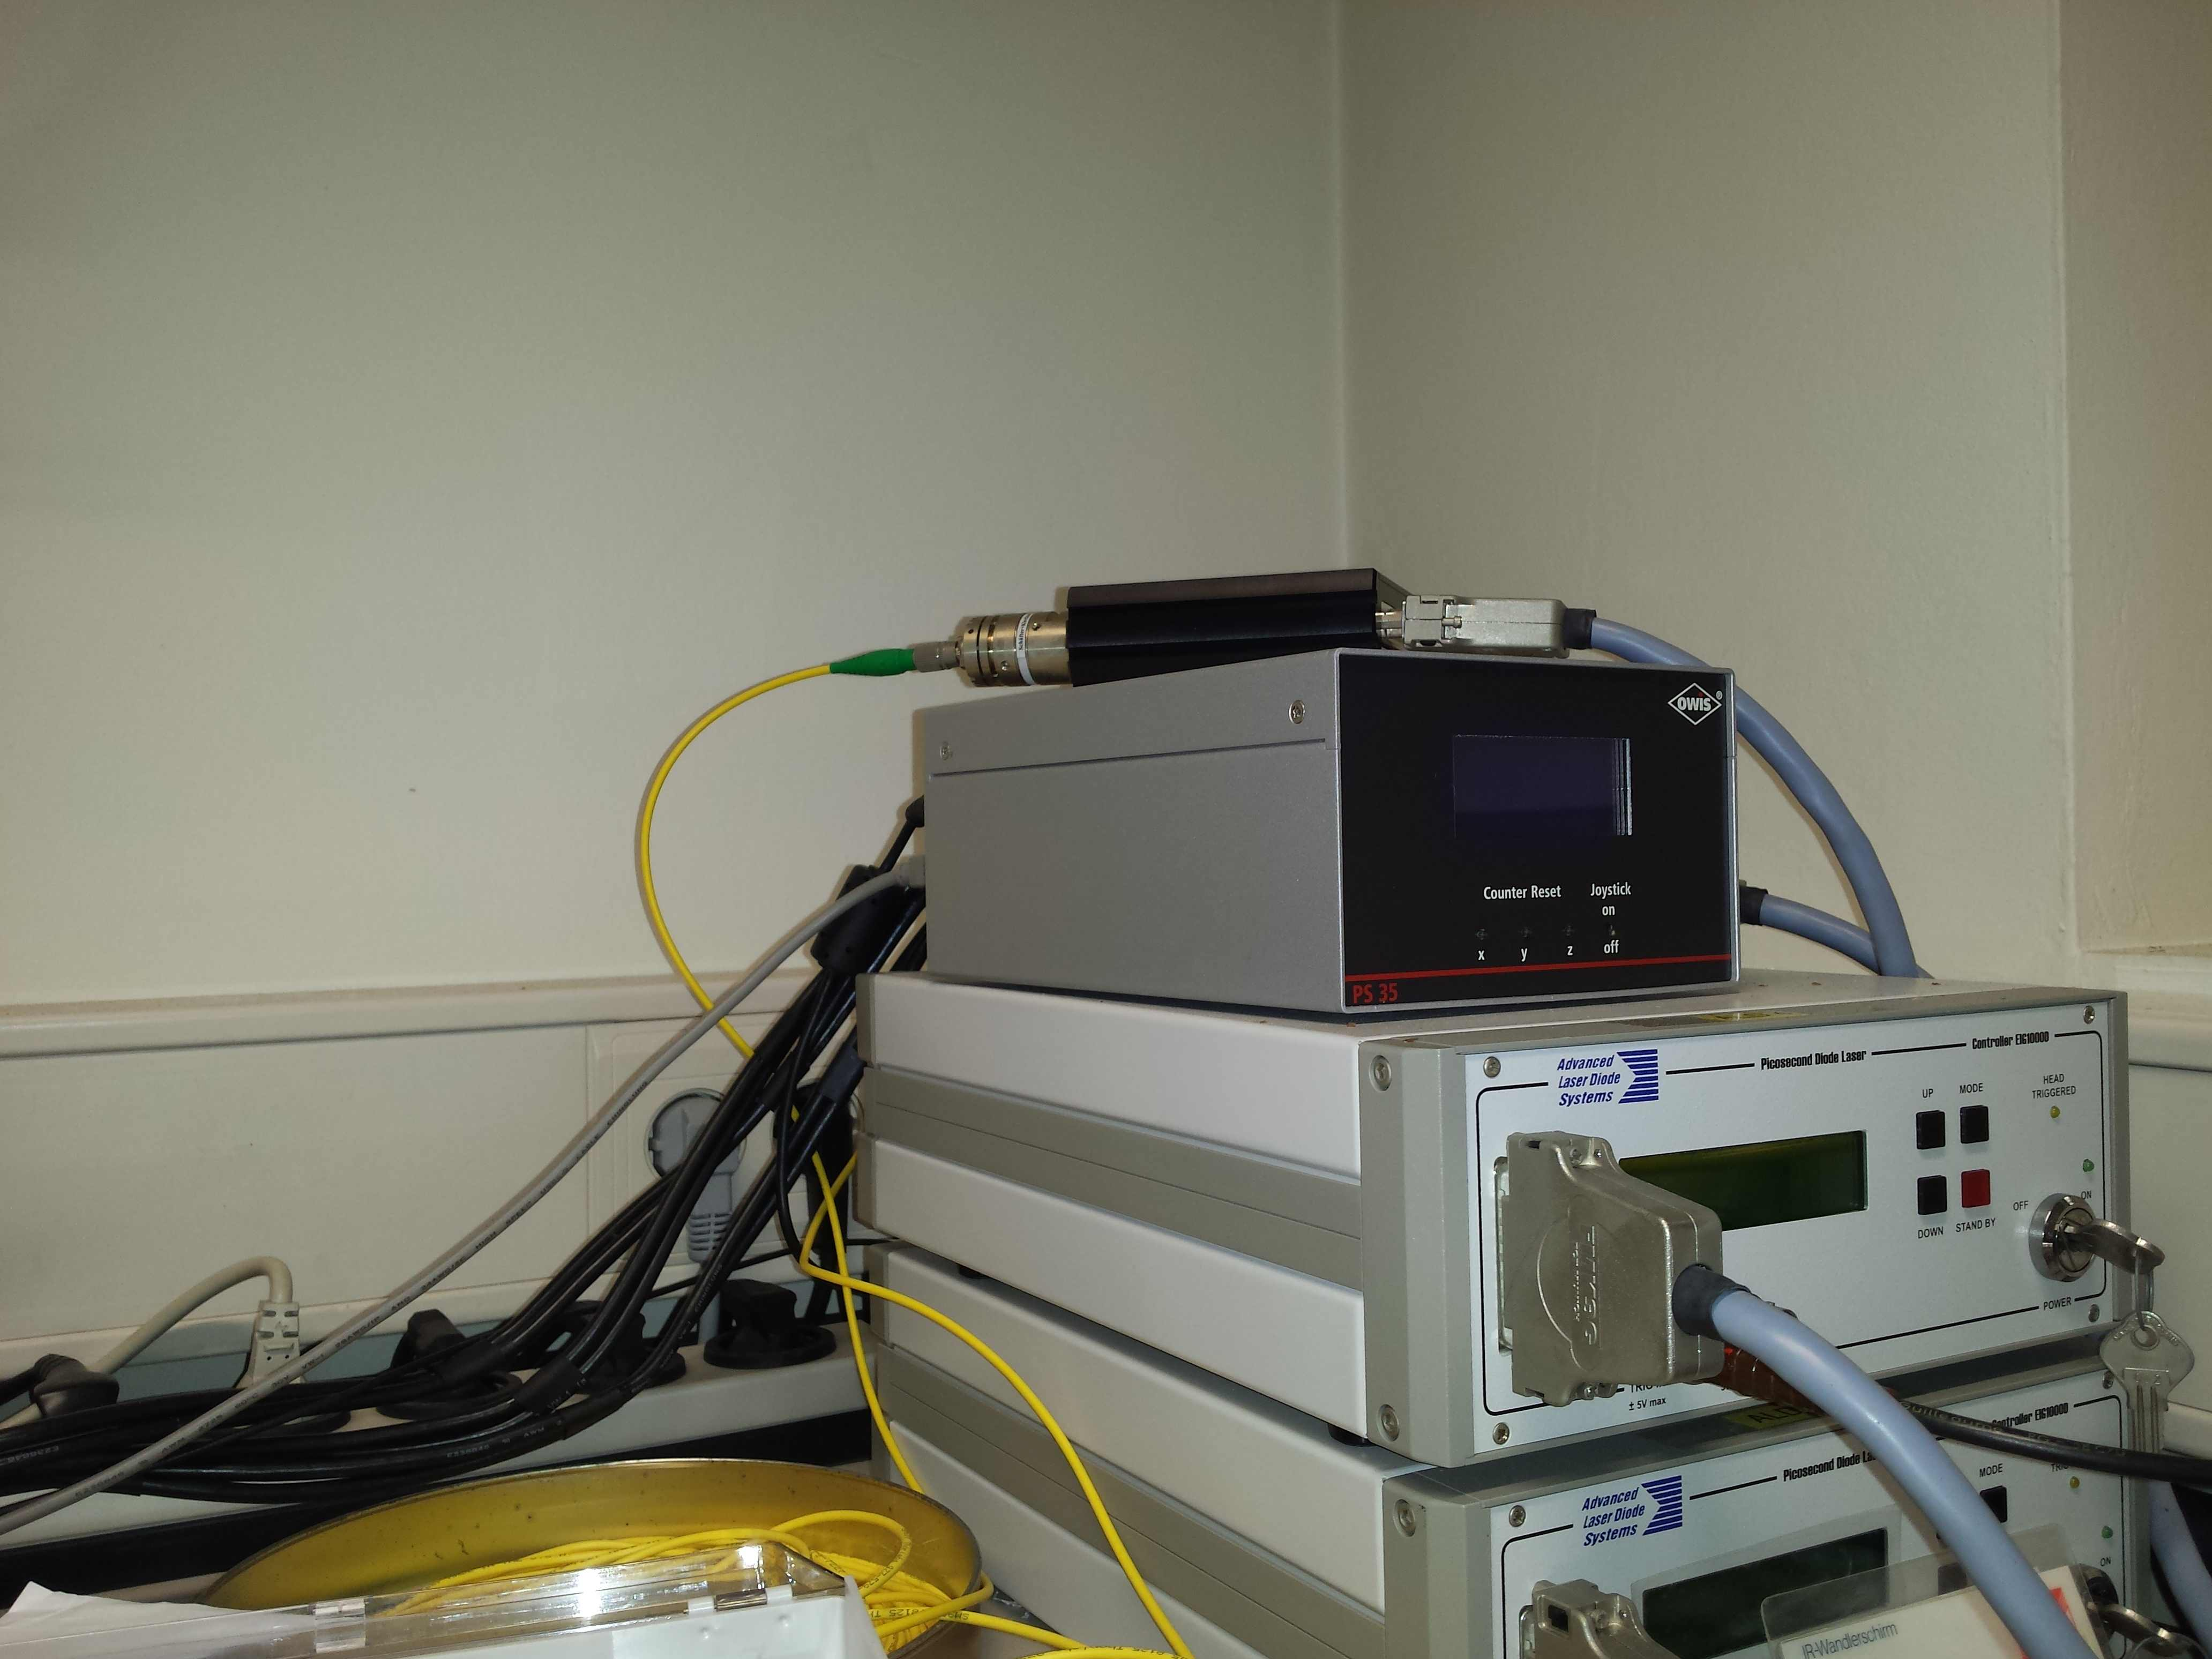
\includegraphics[width=0.32\textwidth]{pictures/DriverTable.jpg}
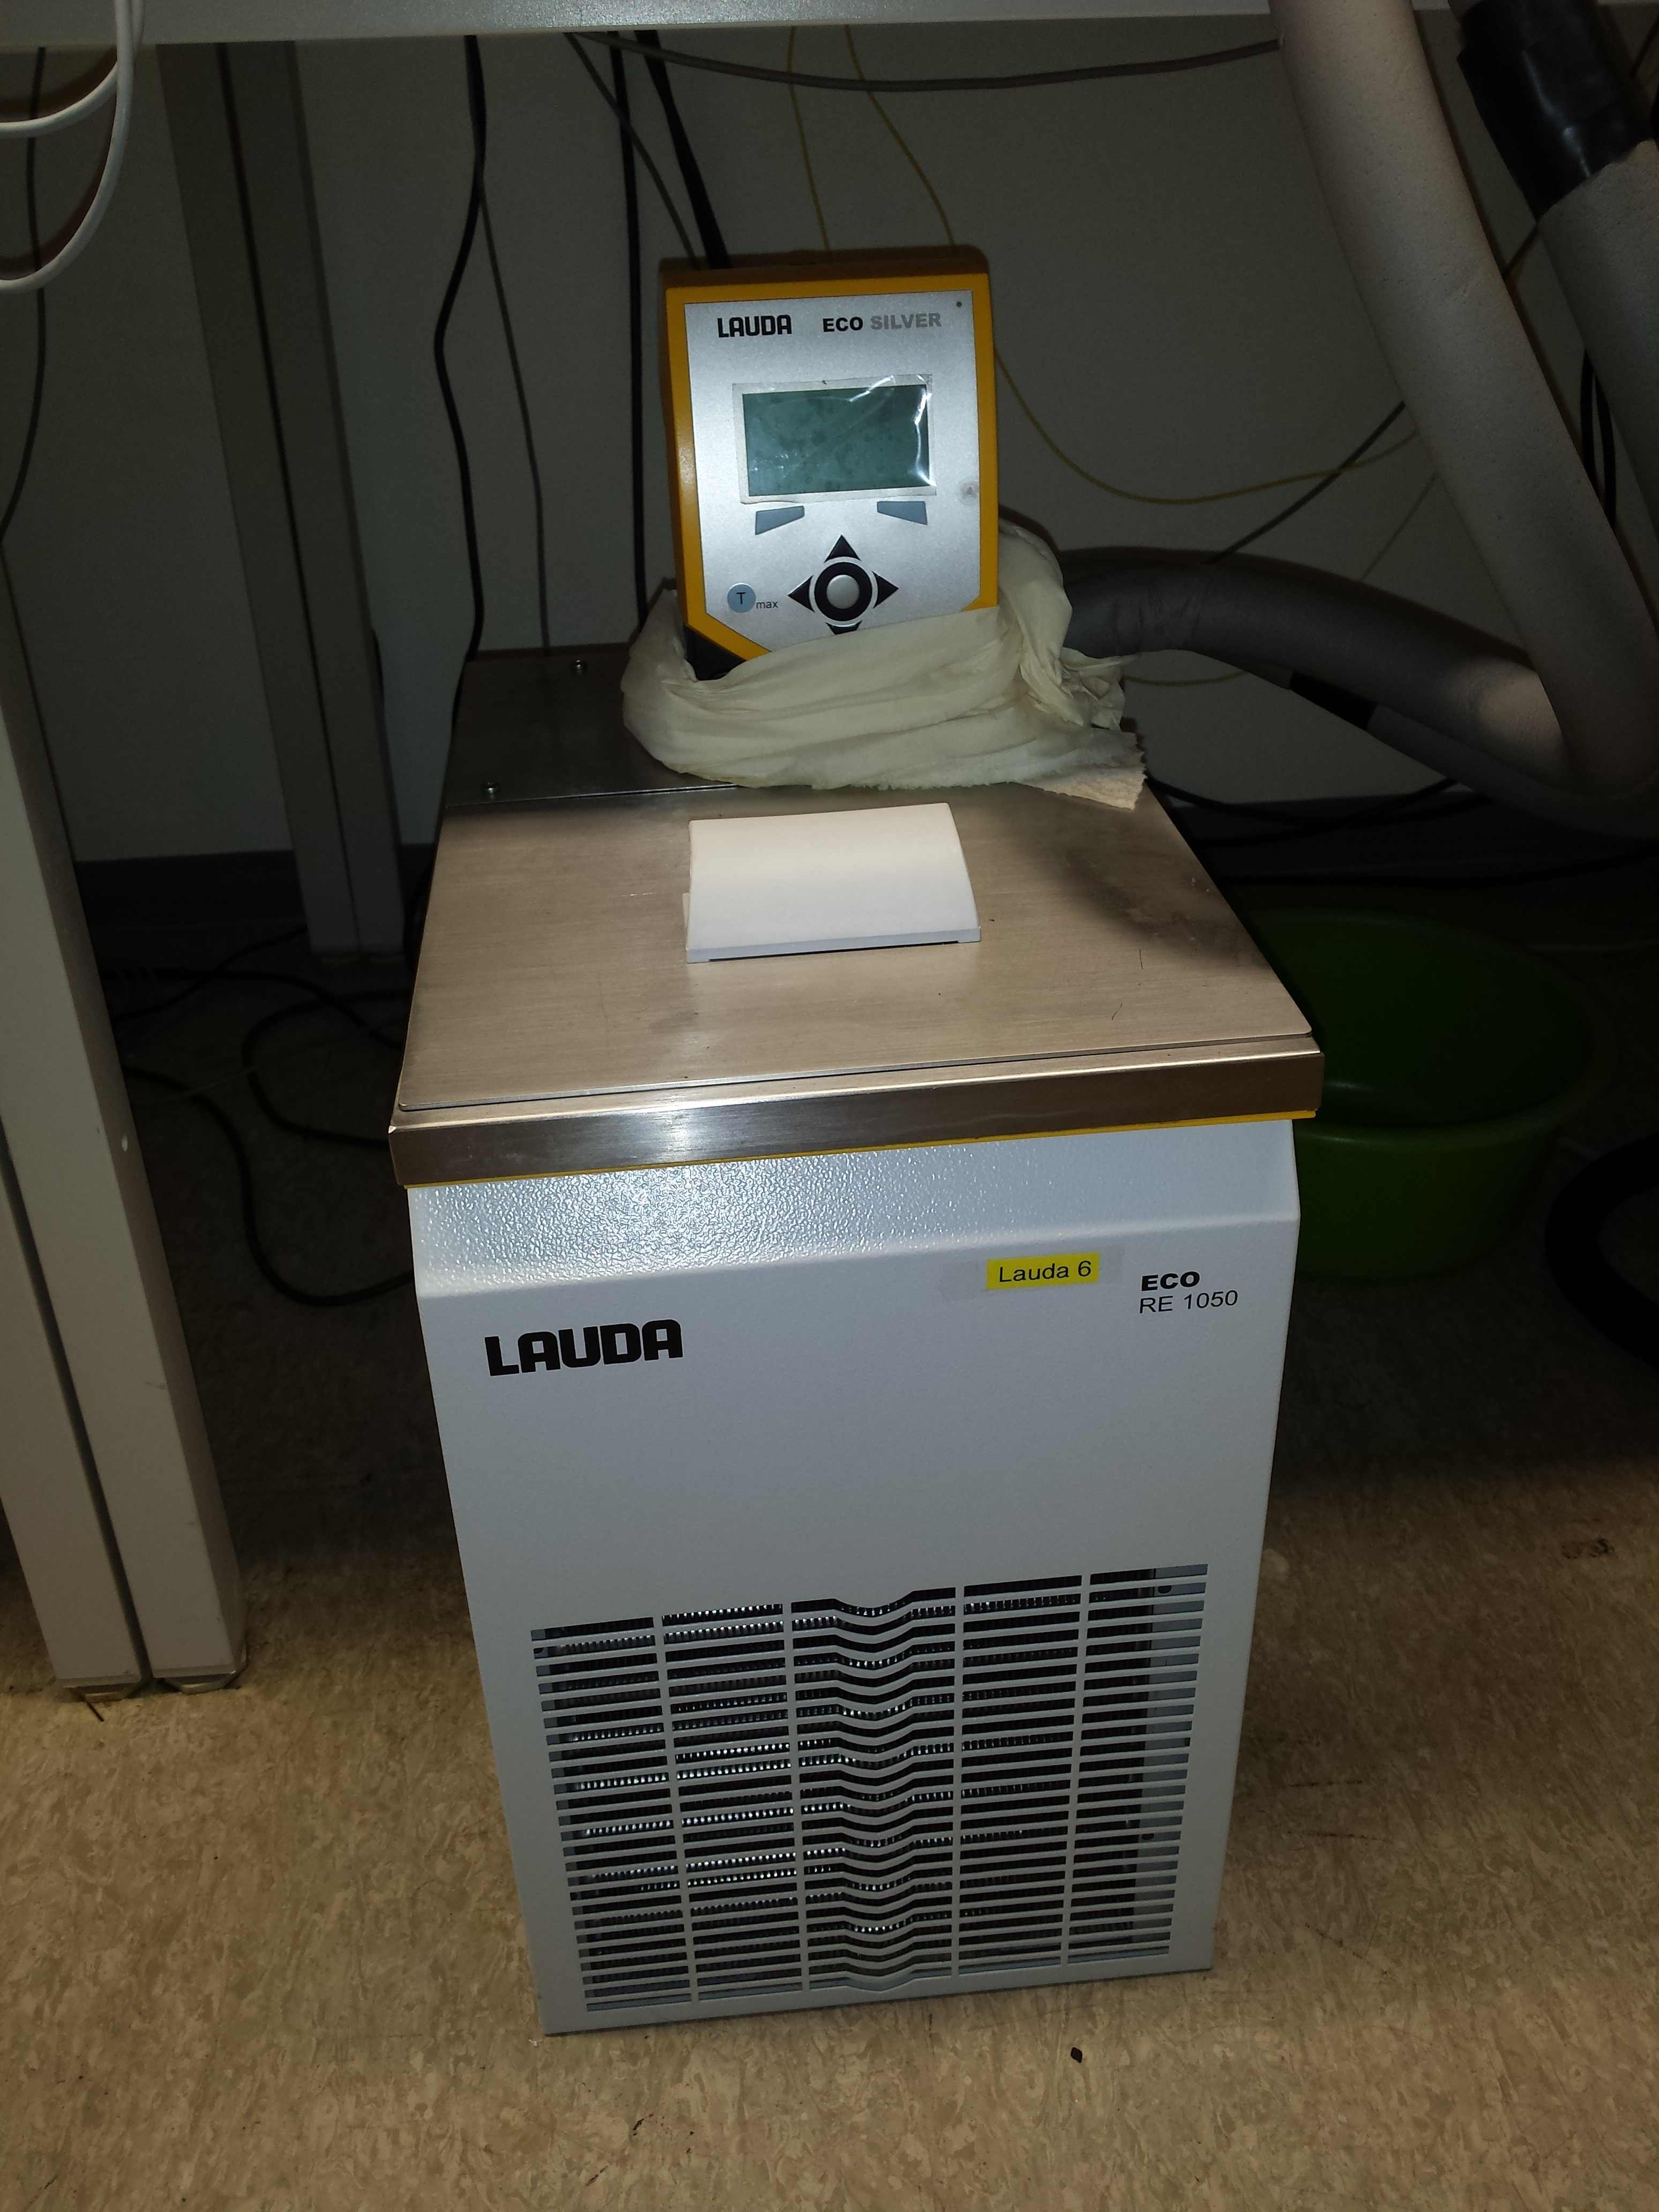
\includegraphics[width=0.32\textwidth]{pictures/HeatExchanger.jpg}
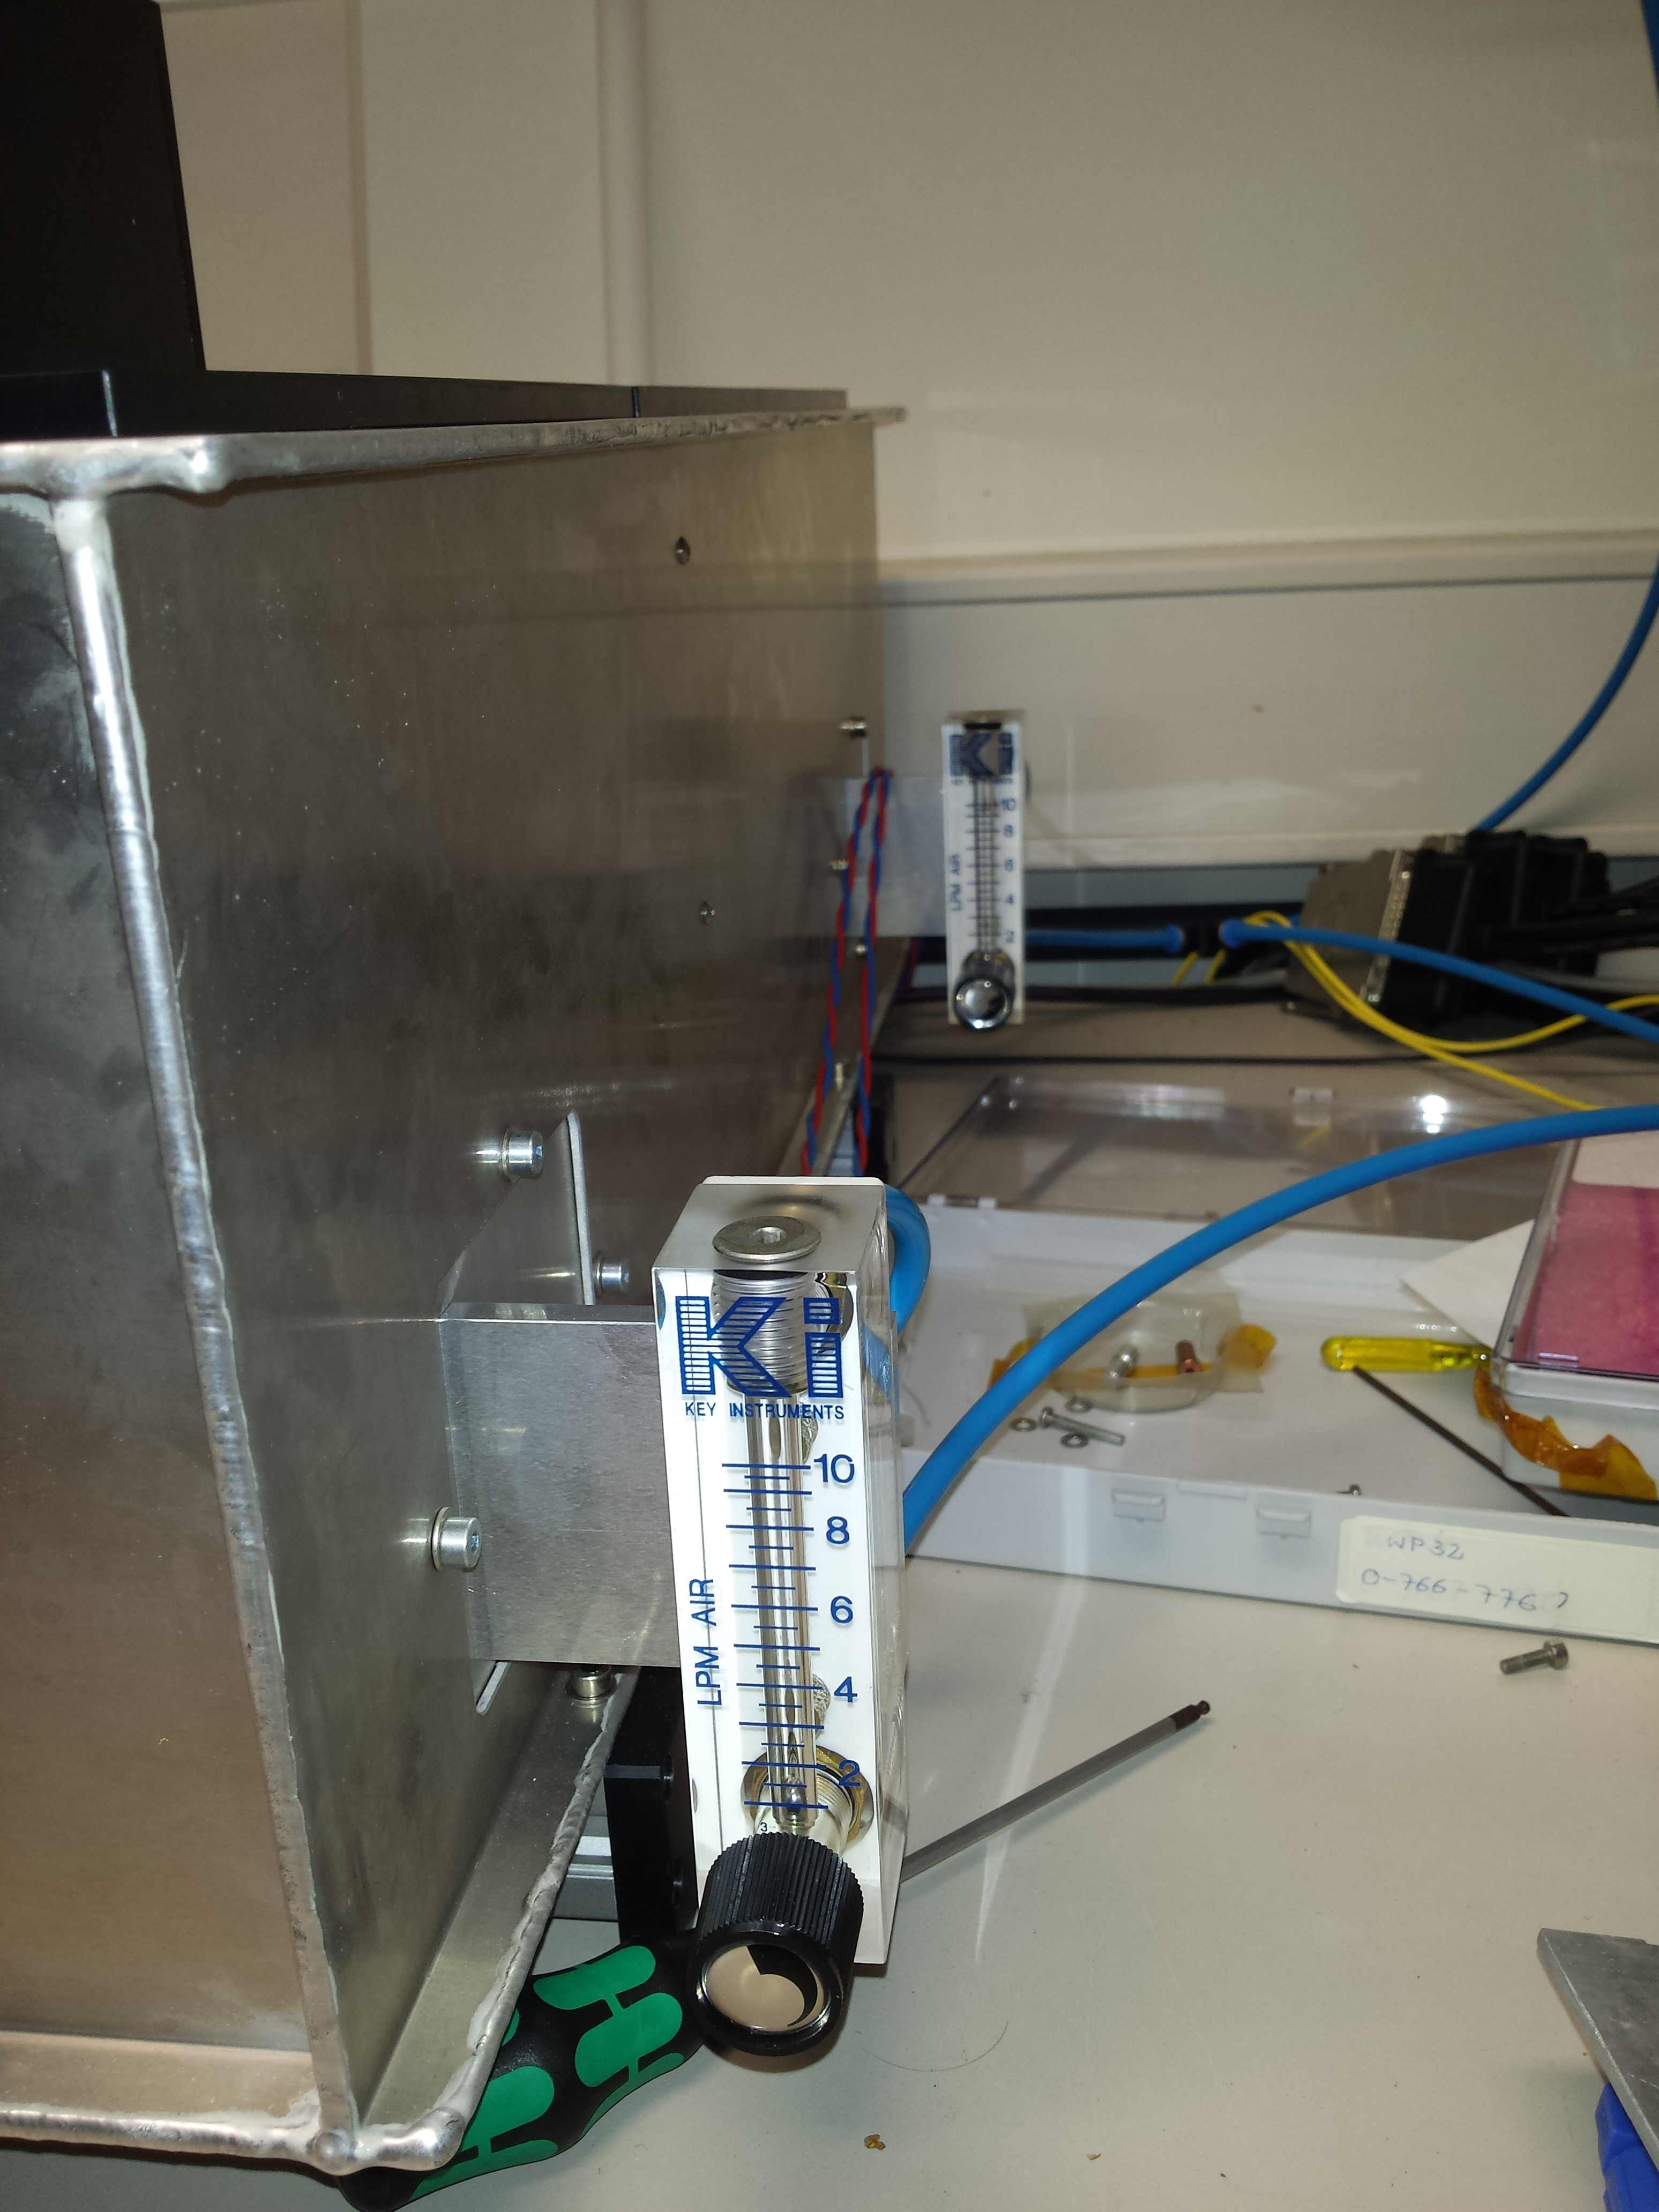
\includegraphics[width=0.32\textwidth]{pictures/DryAirSupply.jpg}
\end{tabular}
\end{center}
\caption{The left picture shows the power supply for the driver of the table(7), in the middle the heat exchanger is shown(8) and on the right the two valves for the dry air supply are visible(9). The numbers in brackets correspond to table \ref{tab:devices}. }
\label{fig:CurrentAndVoltageTrigger}
\end{figure}

\bibliography{Master}{}
\bibliographystyle{plain} 


\end{document}
